%% (REQUIRED) (Thesis including published works only)
%% ACTION
%%      Ensure that your thesis meets the thesis including published works requirements. Some faculties vary requirements in terms of the number of papers required, status of papers and other criteria
%%      Read through and change the details that are in all caps (you should not use all caps in the replacement text)
\Declarationpublication{{}
I hereby declare that this thesis contains no material which has been accepted for the award of any other degree or diploma at any university or equivalent institution and that, to the best of my knowledge and belief, this thesis contains no material previously published or written by another person, except where due reference is made in the text of the thesis.

%% ACTION: Change COUNT, COUNT, THEME, NAME, NAME
This thesis includes COUNT original papers published in peer reviewed journals and COUNT submitted publications.. The core theme of the thesis is THEME. The ideas, development and writing up of all the papers in the thesis were the principal responsibility of myself, the student, working within the \printThesisDepartment under the supervision of NAME and NAME.

%% ACTION: Remove this paragraph for theses with sole-authored work
The inclusion of co-authors reflects the fact that the work came from active collaboration between researchers and acknowledges input into team-based research.

%% ACTION: If this is a laboratory-based discipline, a paragraph outlining the assistance given during the experiments, the nature of the experiments and an attribution to the contributors could follow.

%% ACTION: Insert chapter numbers
In the case of Chapters \ref{chap:article1} and \ref{chap:article2}, my contribution to the work involved the following:

%% ACTION: Update the table to list your publications
%%      The status might be: in press, accepted, returned for revision, submitted
%%      If no co-authors, leave fields blank 
\definecolor{thesisdark}{HTML}{1E1E1E}
\definecolor{thesislight}{HTML}{EEEEEE}
\newcommand{\formatVspace}[1]{\vspace{1ex}{#1}\vspace{1ex}}
\newcommand{\formatH}[1]{\textcolor{thesislight}{\textbf{#1}}}
\newcommand{\formatHv}[1]{\formatVspace{\textcolor{thesislight}{\textbf{#1}}}}
\begin{center}
    \addtolength{\leftskip} {-1cm} %% Fix centering for when table is wider than \textwidth
    \addtolength{\rightskip}{-1cm} %% Fix centering for when table is wider than \textwidth
    \small
    %\footnotesize
    \begin{NiceTabular}[colortbl-like]
            {|c|p{30mm}|c|p{25mm}|p{37mm}|p{25mm}|}
        \hline
        \Block[fill=thesisdark,v-center]{1-1}{\formatH{\makecell{Thesis\\Chapter}}} &
        \Block[fill=thesisdark,v-center]{1-1}{\formatH{Publication Title}} &
        \Block[fill=thesisdark,v-center]{1-1}{\formatH{Status}} &
        \Block[fill=thesisdark,v-center]{1-1}{\formatH{Nature and \% Student Contribution}} &
        \Block[fill=thesisdark,v-center]{1-1}{\formatHv{Co-author name(s) Nature and \% of Co-author's contribution}} &
        \Block[fill=thesisdark,v-center]{1-1}{\formatH{Co-author(s), Monash student}}\\

        %% ACTION: The number of co-authors must be reflected in \Block[v-center]{4-1}
        %%    i.e. change the number 4 to the number of co-authors
        %%    This defines how big the multi-row block is
        \hline
        \Block[v-center]{4-1}{\ref{chap:article1}} &
        \Block[v-center]{4-1}{\formatVspace{The Title of My First Published Article}} &
        \Block[v-center]{4-1}{Published} &
        \Block[v-center]{4-1}{(70\%)} &
        \Block[v-center]{1-1}{\formatVspace{NAME: contribution~1, contribution~2 (10\%)}} & \Block[v-center]{1-1}{No}\\
        \cline{5-6}
        &&&&\Block[v-center]{1-1}{\formatVspace{NAME: contribution~1, contribution~2 (10\%)}} & \Block[v-center]{1-1}{No}\\
        \cline{5-6}
        &&&&\Block[v-center]{1-1}{\formatVspace{NAME: contribution~1 (5\%)}} & \Block[v-center]{1-1}{No}\\
        \cline{5-6}
        &&&&\Block[v-center]{1-1}{\formatVspace{NAME: contribution~1 (5\%)}} & \Block[v-center]{1-1}{No}\\

        %% ACTION: The number of co-authors must be reflected in \Block[v-center]{2-1}
        \hline
        \Block[v-center]{2-1}{\ref{chap:article2}} &
        \Block[v-center]{2-1}{\formatVspace{The Title of My Second Published Article}} &
        \Block[v-center]{2-1}{In Press} &
        \Block[v-center]{2-1}{(80\%)} &
        \Block[v-center]{1-1}{\formatVspace{NAME: contribution~1, contribution~2 (10\%)}} & \Block[v-center]{1-1}{No}\\
        \cline{5-6}
        &&&&\Block[v-center]{1-1}{\formatVspace{NAME: contribution~1, contribution~2 (10\%)}} & \Block[v-center]{1-1}{No}\\
        \hline
    \end{NiceTabular}
\end{center}

I have not renumbered sections of submitted or published papers in order to generate a consistent presentation within the thesis.

\textbf{Student name:} \printThesisAuthor

%% OPTIONAL: Choose how to display the date
%%      For more options, see the package 'datetime'
\ddmmyyyydate
%\yyyymmdddate\renewcommand{\dateseparator}{-}

%% ACTION: Add your signature file
\textbf{Student signature:}\hspace{3mm}%%
\raisebox{-.5\height}{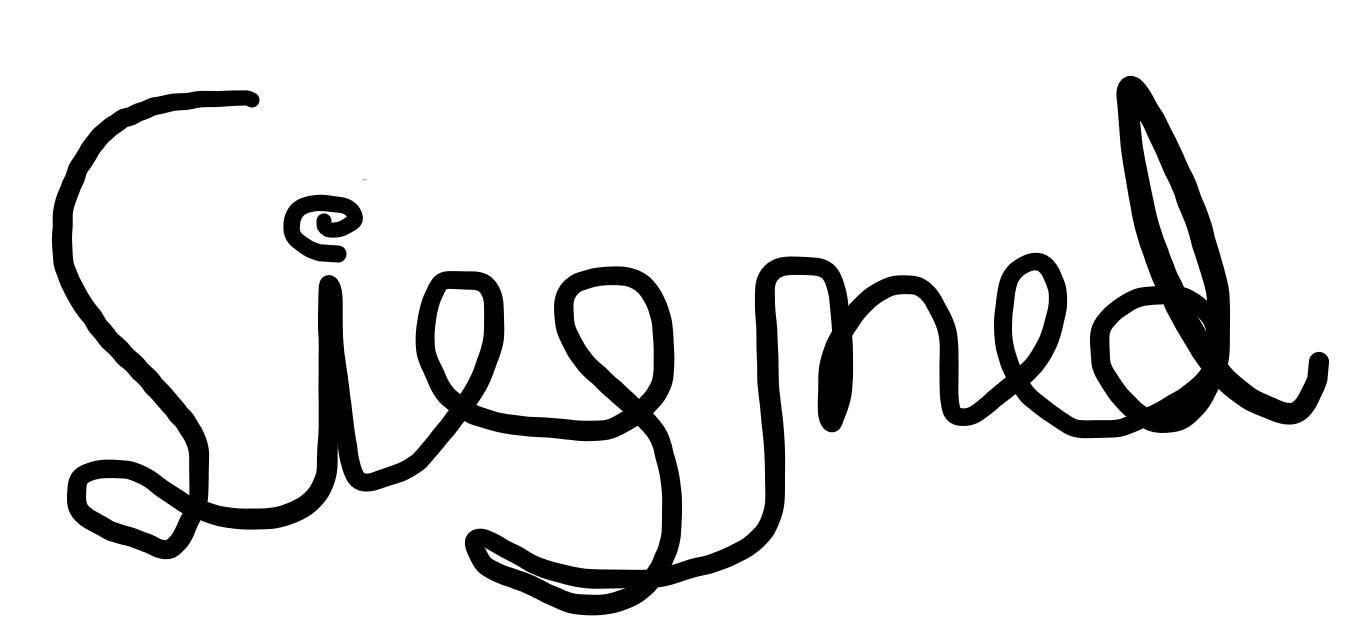
\includegraphics[height=2.5em,keepaspectratio]{Figures/SignatureMe.png}}%%
\hfill%%
\textbf{Date:} \today

I hereby certify that the above declaration correctly reflects the nature and extent of the student's and co-authors' contributions to this work. In instances where I am not the responsible author I have consulted with the responsible author to agree on the respective contributions of the authors.

%% ACTION: Add your main supervisor's name and signature file
\textbf{Main Supervisor name:} NAME

\textbf{Main Supervisor signature:}\hspace{3mm}%%
\raisebox{-.5\height}{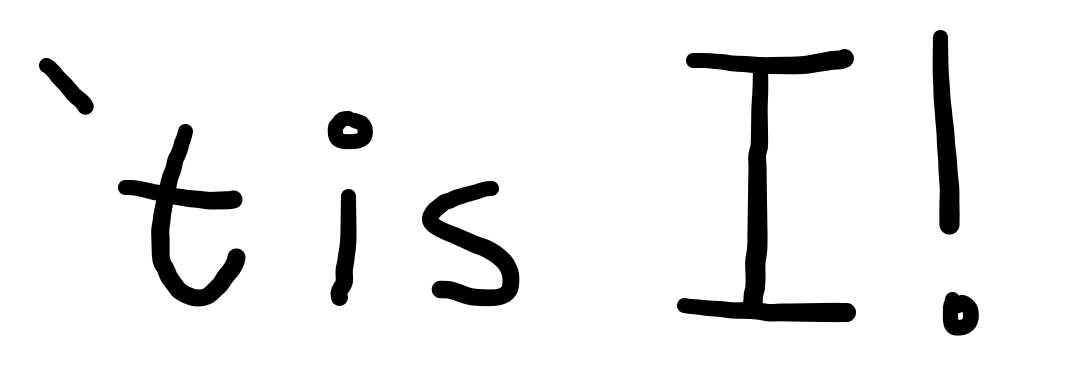
\includegraphics[height=2.5em,keepaspectratio]{Figures/SignatureSupervisor.png}}%%
\hfill%%
\textbf{Date:} \today


}